\documentclass[twocolumn]{svjour3}[2016]

\usepackage{graphicx}
\usepackage{cite}
\usepackage{subfig}
\usepackage{mathtools}
\usepackage{amsmath}
\usepackage{amssymb}
\usepackage{tabularx}
\usepackage{hhline}
\newcolumntype{/}{!{\vrule width 2pt}}
\newcolumntype{Y}{>{\centering\arraybackslash}X}

\begin{document}
%HEADER
\title{Exploring Unstructured Environment with Frontier Trees}
\author{R. Korb \and A. Schoettl}
\institute{
	Rudolf F. S. Korb \at
	University of Applied Sciences - Munich\\ Dept. 04 Electrical Engineering and Information Technology, Laboratory for Autonomous Systems in Munich (LASIM),  Lothstr. 64, 80335 Munich, Germany\\Tel.: +49-89-1265-3415\\
	\email{rudolf.korb@hm.edu}
	\and
	Alfred Schoettl \at
	University of Applied Sciences - Munich\\ Dept. 04 Electrical Engineering and Information Technology, Laboratory for Autonomous Systems in Munich (LASIM),  Lothstr. 64, 80335 Munich, Germany\\Tel.: +49-89-1265-3415\\
	\email{alfred.schoettl@hm.edu}
}

\maketitle

\begin{abstract}
\textbf{
%\textit{
	This paper presents the Frontier Tree exploration algorithm, a novel approach to autonomously explore unknown and unstructured areas. Focus of this work is the exploration of domestic environments with arbitrary obstacles, for example furbished appartements. Existing and well studied approaches like greedy algorithms perform worse, when obstacles are included and the range of distance sensors is limited. Base of this research is the Frontier Tree. This data structure offers two main features. It is a memory of past poses during exploration and is utilized to decide between future navigation goals. This approach is compared to a basic but efficient nearest neighbour exploration. The algorithm is tested in simulation with maps similar to appartement ground maps including furniture as obstacles. The paper shows, that frontier trees minimize the travelled path of the mobile robot by tracking open boundaries.

}
\keywords{Robotics \and  Exploration \and  Path Planning \and  Frontiers \and Domestic Environment}
\end{abstract}

\section{Introduction}
\label{introduction}
Mobile robots must be familiar with their surroundings to execute complex tasks, for example pick-up and delivery services. As an initial step, the workspace has to be explored autonomously. This problem can be divided into three parts; mapping, localization and exploration. Focus of this research is planning future exploration steps to uncover the environment efficiently, depending on past steps, a map of the area already explored and the agent's current position.\\
When robots participate in everyday life, their operation space consists of unstructured, dynamic environments and has to deal with interieur and crowded areas.
As a consequence, when service robots operate in private appartements or public buildings like hospitals or retirement homes, they need to adapt itselves to their surroudings.
Therefore it is crucial for a mobile robot to explore areas autonomously and not rely on an environment designed specifically for a service device.\\
Basic algorithms follow a greedy approach to select future robot positions during the exploration problem. These approaches use the robot's current state and plan one step ahead by minimizing a cost function, for example the agent's euclidian distance to a boundary of known and unknown space. For exploration of simple maps, unfurbished rooms and corridors, basic algorithms provide acceptable results, depending on for example sensor constraints. With high range distance sensors and obstacle free areas, robots cover the entire room before leaving and most likely do not create open boundaries. Therefore, rooms do not have to be visited again and the traveled distance is less compared to low range sensing robots. Furthermore, the number of possible decisions to choose the next goal from is rising with the environment's complexity. As a result, the greedy algorithm's performance will decrease. The robot has to revisit parts of the map where boundaries have been forgotten, increasing the traveled distance.\\
Consequently the two main influences for travelling distance during exploration is the complexity of an agent's environment and constraints of its range sensors. Mobile autonomous robots in unstructered environment are dealing with both, high complexity and sensor limitations. Many algorithms use maps with reduced difficulty, expecting an empty environment or assume a sensor with infinite distance measurements. It follows, that algorithms covering only one impact decrease in efficiency, when a complex environment and sensor limitations are present.\\
Greedy algorithms dealing with both influences have one major flaw, which leads to a rise of traveled distance and exploration time. Approaching a boundary already discovered several steps ahead, is an indication that the robot's current exploration path is a cycle. As a result, open boundaries between the starting and endpoint of the cycle will be reached with high travel costs later on during the exploration task. The frontier tree recognizes cycles and hence is able to avoid high costs and react early on forgotten boundaries.

% For one-column wide figures use
%\begin{figure}
%  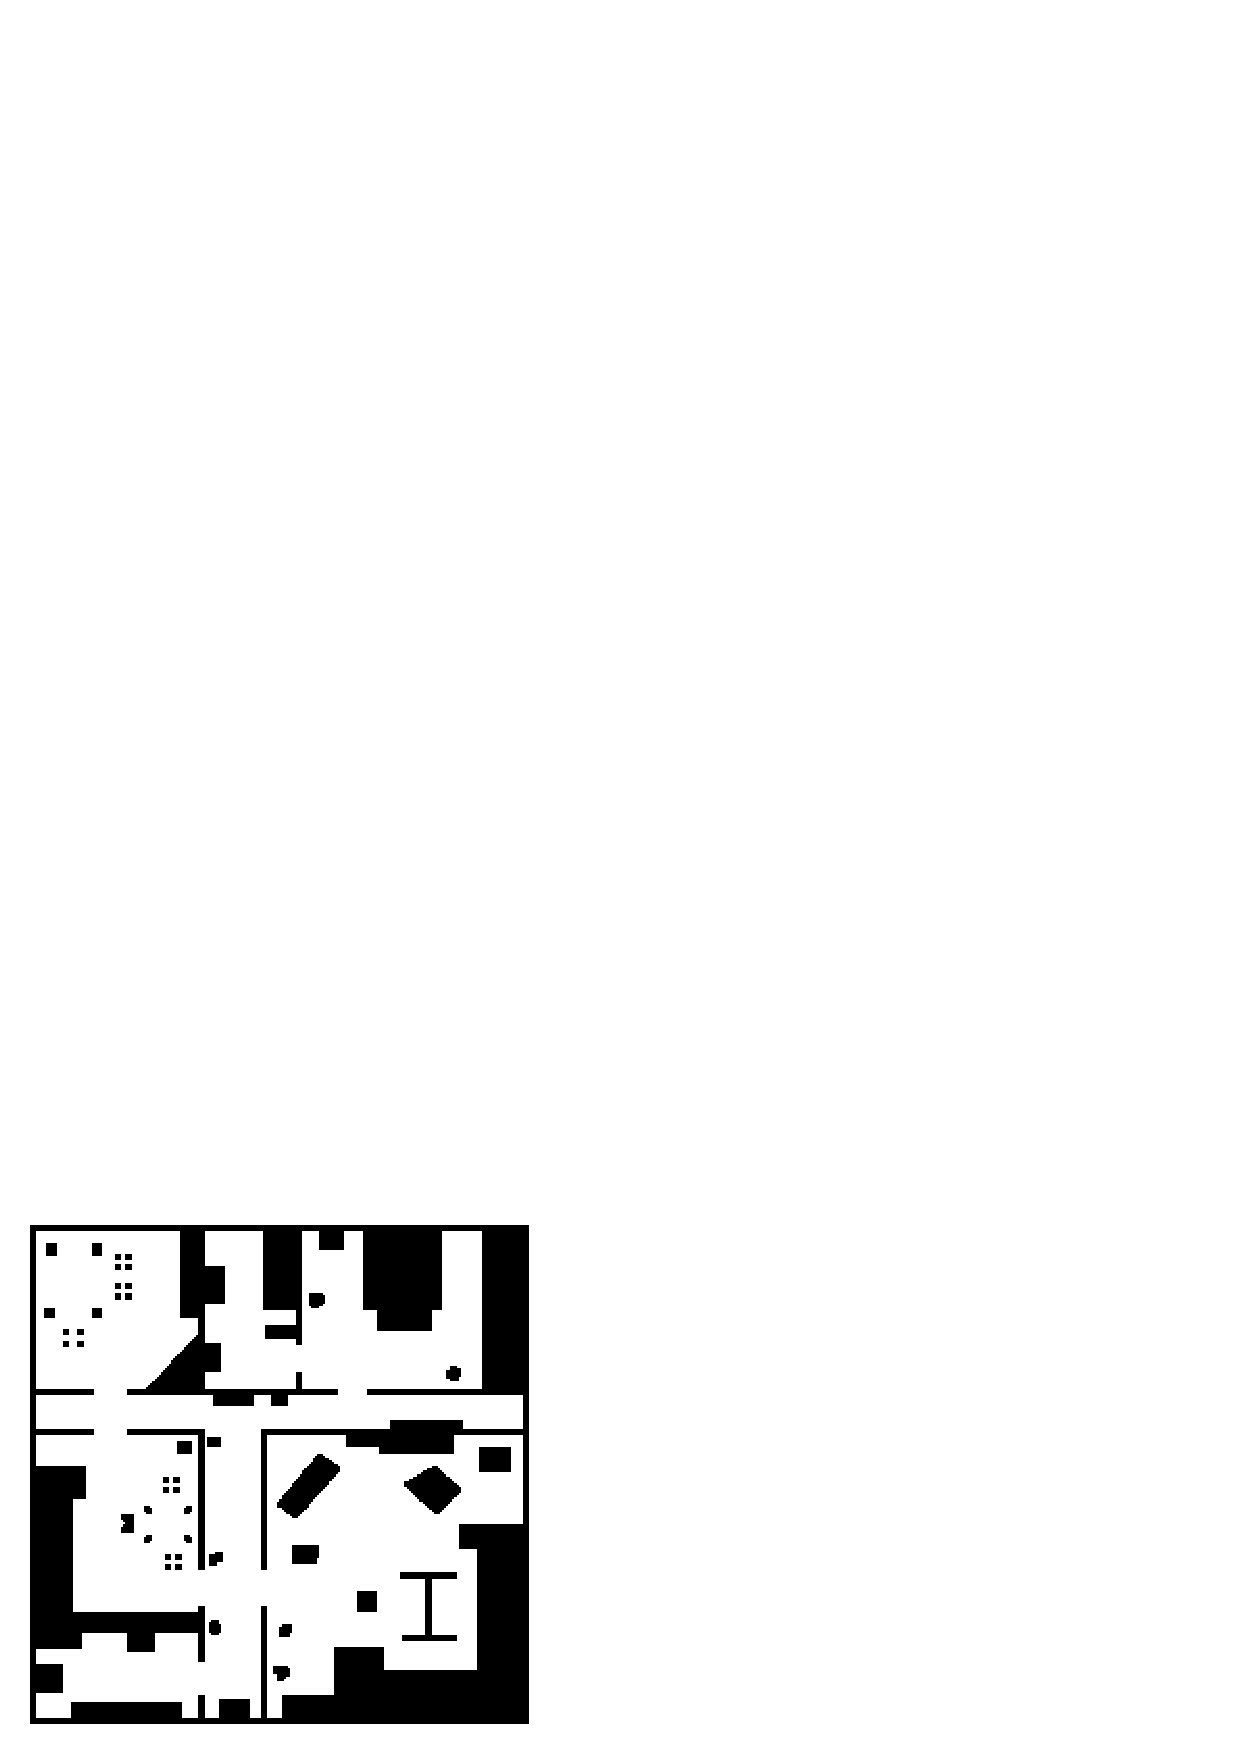
\includegraphics[width=5cm,height=5cm]{map_19.pdf}
% figure caption is below the figure
%\caption{Please write your figure caption here}
%\label{fig:1}       % Give a unique label
%\end{figure}

\section{Related Work}
\label{related_work}
Many exploration algorithms use the frontier approach introduced by Yamauchi \cite{brian_yamauchi_frontier-based_2007}. A frontier is defined as the boudary between known and unknown space in the currently explored map. The algorithm proposed in this paper also utilizes frontiers as atomic elements in the tree data structure and are discussed in detail in section \ref{frontiers}. Yamauchi's exploration algorithm is a greedy approch and chooses the shortest obstacle free path to minimize the distance between a robot's position and the next frontier.\\
Koenig et al. \cite{sven_koenig_greedy_2001} show, that greedy algorithms explore ares with acceptable results. For improvements, map segmentation algorithms were introduced \cite{dirk_holz_evaluating_2010, kai_m._wurm_coordinated_2008} to reduce the travel distance of greedy approaches. Wurm et al. \cite{kai_m._wurm_coordinated_2008} use Voronoi Graphs to divide the explored environment in segments. While large emtpy spaces are segmented well, narrow areas, for example corridors, yield a vast amount of partitions. As a result, the disadvantage of greedy algorithms remains. Holz et al. \cite{dirk_holz_evaluating_2010} extend the segmentation by adding a step for merging several partitions.\\
To keep track of open boundaries, Nasir and Elnagar \cite{reem_nasir_gap_2015} use a data structure called Gap Navigation Tree, introduced by Tovar et al. \cite{benjamin_tovar_optimal_2003}.\\
Another approach is using information based heuristics \cite{arnoud_visser_balancing_2008,amir_mobarhani_histogram_2011,robert_grabowski_autonomous_2003}. Visser and Slamet \cite{arnoud_visser_balancing_2008} minimize information entropy by selecting frontiers with the largest area. Additionally, they consider travel distance to each frontier in their cost function, to increase the algoritm's efficiency. In \cite{amir_mobarhani_histogram_2011}, Mobarhani et al. also discuss the tradeoff between an information based heuristic and travel distance. They count the number of points of all frontiers at an angle interval from the robot's current position and fill an angle histogram. The next best frontier is selected with a weighted cost funtion by maximising the number of frontier cells at a specific direction and minimizing the travel time to the frontier.\\
Information based approaches are especially good for rescue scenarios.Focus of these algorithms is uncovering large parts of the map quickly. It is possible that these heuristics result in alternating poses between opposite parts of the map. This behaviour leads to an increased travel distance.\\
%Exploration by a team of mobile robots is also investigated intensively \cite{antonio_franchi_sensor-based_2009,andreas_nuchter_enhanced_2015,cyrill_stachniss_efficient_2008,kai_m._wurm_coordinated_2008,robert_grabowski_autonomous_2003} but is not part of the research in this paper.

\section{Outline}
\label{outline}
%The worst case of greedy algorithms is not optimal, but the difference to the worst case optimal travel distance is reasonable small.
Although the difference to between the worst case of greedy algorithms and the worst case optimal travel distance is reasonable small, the performance is reduced with rising map complexity and sensor limitations.
A major weakness of an efficient greedy algorithm is illustrated in figure \ref{fig:1}. When entering a room with obstacles, it is possible, that the robot runs in a cycle and returns to a previous area before finishing the room. This behaviour results in higher travel cost, because the robt has to revisit the room. Segmentation approaches \cite{dirk_holz_evaluating_2010, kai_m._wurm_coordinated_2008} to further reduce travel cost, highly rely on the geometrical appearence of the map. With an environment containing obstacles, the probability of revisiting a room is increasing. Segmentation in combination with merging minimizes the number of segments, but does not eliminate the problem, where the robot's path is in a cycle.\\
With Gap Navigation Trees Tovar et al. \cite{benjamin_tovar_optimal_2003} solve the problem of map complexity with arbitrary obstacles, but assume infinite distance measurement und $360^{\circ}$ opening angle and therefore do not have sensor constraints. A reduced map size grants this property for real life experiments.\\
The exploration algorithm proposed in this paper performs well with complex structure and sensor limitations. It offers the ability to react, when the agent runs in a cycle to prevent further travel cost.

\begin{figure}
  \includegraphics{figures/fig1.pdf}
% figure caption is below the figure
  \caption{
  This illustration shows six robot states during exploration, following a greedy algorithm. The robot enters a room with obstacles and leaves before uncovering the whole area. As a result, the agent has to return at a later exploration step.}
  \label{fig:1}       % Give a unique label
\end{figure}

%Another approach is adding a second cost function to the exlporation algorithm \cite{arnoud_visser_balancing_2008}.
\section{The Frontier Tree Algorithm}
\label{tfta}

Foundation of this exploration algorithm is a tree data structure with frontiers as nodes. The definition of a frontier is related to Yamauchi's approach \cite{brian_yamauchi_frontier-based_2007}. Similar to Gap Navigation Trees \cite{benjamin_tovar_optimal_2003}, the data structure is, inter alia, used for tracking open boundaries during exploration. Additionally, the resulting topological tree map is used to select the next exploration goal. The final path planning to the new pose is executed on a 2D grid map.


\subsection{Robot Model}
In this paper the robot is implemented as mobile base with a circular footprint and three degrees of freedom. The position and orientation is defined by $\textbf{r} = (x, y, \theta)^{T}$ with $x, y$ as position and $\theta$ as orientation. Additionally, the agent provides a distance sensor, represented by $\textbf{s} = (d, \alpha)^{T}$. Component $d$ is the sensor's range and $\alpha$ its opening angle. As an assumption, the robot is able to localize itself on a 2D grid map using a simultaneous localization and mapping (SLAM) approach.

\subsection{Map Representations}
To fulfill the exploration task, the algorithm uses five maps of three different types. A basic map type is the occupancy grid map with values between $0$ and $1$, where white pixels ($1$) mark free and black pixels ($0$) unpassable space. Values in the interval $(0,1)$ can be interpreted as unknown space. An oocupancy map is the output of a SLAM algorithm. Unpassable pixels are inflated by the radius of the robot's footprint, resulting in a global occupancy map $\textrm{occ}_g$ where the agent can be treated as a point. $\textrm{occ}_g$ is used to create a local (with dependency of $\textbf{r}$) occupancy map $\textrm{occ}_{l}$.
\begin{equation}
%\[
\textrm{occ}_ {l}(\textbf{x})=
\begin{dcases}
0.5, & \text{if } \textrm{dist}(\textbf{x}, \textbf{r}) \geq l\\
\textrm{occ}_{g}(\textbf{x}), & \text{otherwise}
\end{dcases}
%\]
\end{equation}
where $\textrm{dist}(\textbf{x}, \textbf{r})$ is the euclidian distance between the considered pixel $\textbf{x}$ in $\textrm{occ}_{local}$ to the current robot position $\textbf{r}$.
\\
Both, $\textrm{occ}_{g}$ and $\textrm{occ}_{l}$, as well as the current pose $\textbf{r}$ are utilized for the calculation of global and local cost maps $\textrm{cost}_{g}$ and $\textrm{cost}_{l}$. These are calculated with Dijstra's Algorithm. Without a return criterion, the result is a map with the $\textrm{cost}(\textbf{x})$ to travel from $\textbf{r}$ to $\textbf{x}$.\\
Lastly, $\textrm{occ}_g$ is used to create a frontier map $\digamma$, containing the possible future goals for exploration. Since $\textrm{occ}_g$ is an inflated representation, every point in $\digamma$ is a possible navigation goal. Section \ref{frontiers} gives a formal description of frontiers.

\begin{figure}
\centering
  \mbox{
  \subfloat[Occupancy map]{
    %\includegraphics{figures/fig2a.pdf}
    \includegraphics[width=39mm]{figures/occupancy_map_13.png}
    \label{fig2:a}
  }
  \subfloat[Frontier map]{
      %\includegraphics{figures/39.pdf}
      \includegraphics[width=39mm]{figures/frontier_map_13.png}
      \label{fig2:b}
    }
  }
    \mbox{
    \subfloat[Cost map]{
      %\includegraphics{figures/fig2c.pdf}
      \includegraphics[width=39mm]{figures/rmap_14.png}
      \label{fig2:c}
    }
    \subfloat[Local cost Map]{
        %\includegraphics{figures/fig2d.pdf}
        \includegraphics[width=39mm]{figures/local_map_14.png}
        \label{fig2:d}
      }
    }
% figure caption is below the figure
  \caption{(a)The Occupancy map displays the knowledge of the robot about its surroundings with white pixels as free, black as occupied and grey as unknown space. (b)Exploration goals for the next steps are displayed in the Frontier Map. (c)The Cost Map combines information about travel cost and reachable points. Pure black is not reachable and travel cost rise with the brighness. (d)The local cost map shows travel cost and reachable points from \textbf{r} to a distance $d + \sigma$ around the robot. }
  \label{typical_map_representations}       % Give a unique label
\end{figure}

\subsection{Frontiers}
\label{frontiers}
Frontiers are extracted from the global occupancy map. A Frontier $f^i$, with index $i$ as unique id, is the boundary between unknown and free space in $occ_g$\cite{brian_yamauchi_frontier-based_2007}. An elementary part of frontier $f^i$ are frontier cells $f^i_j$, where superscript $j$ denotes the index of the single cell inside the frontier. A cell is defined by the following two properties:
\begin{equation}
\textrm{occ}_{g}(\textbf{x}) = 1
\end{equation}
\begin{equation}
\exists\; \textrm{occ}_{g}(\textbf{y})\in N_8(\textbf{x}):\textrm{occ}_{g}(\textbf{y})=(0,1)
\end{equation}
%\begin{equation}
%A\land B\Rightarrow \textbf{x} = f^i_j\text{,}
%\end{equation}
with $N_8$ as the Moore Neighbourhood of index $\textbf{x}$ in occupancy map $\textrm{occ}_g$. Adjacent frontier cells are merged to a single frontier $f^i$. $\mathbb{F}$ is the set of all frontiers $f^i$. Every frontier must specify a cell $f^i_g$ that declares a navigation goal to plan a path from \textbf{r} to $f^i$. This position is given as
\begin{equation}
f^i_g = \textrm{min}(\|f^i_j - \bar{f^i}\|_2)\text{,}
\end{equation}
The frontier cell with the minimum euclidian distance from $f^i_j$ to the mean value of all frontier cells $\bar{f^i}$ is selected.

\subsection{Tree Structure}
Root of the tree structure is the initial position $\textbf{r}_{init}$ of the robot on the map. Each node $n$ has a connection to its parent and contains a list of all children. These links offer the ability to traverse the tree in both directions. The number of a node's descendants is dependent on $\textbf{r}\text{ and }\textrm{cost}_l$. Additionally, every $n_i$ saves $f^i_g$ as data element, representing the navigation goal of the node. Every node can be in one of the three states unmarked, marked or visited. Unmarked nodes are possible goal position for exploration. Marked nodes are a substitution for a delete operation and are not used anymore for the future planning process. A visited node is every node, that has been chosen as exploration goal. In Summary, the frontier tree stores every node thas was a possible goal, all current reachable nodes and contains the complete exploration path. As long as the agent follows frontiers in the same direction, the tree is growing in depth. When the robot has to decide between two or more directions, a subtree is generated and the frontier tree is growing in breadth.
For basic operations on the tree, e.g. traverse the data structure, a breadth first search was implemented.

\subsection{Tree Operations}
\label{tfta:operations}
The Frontier Tree offers two basic operations to directly manipulate the data structure. An Insert function extends the existing children of a node by attaching an element. Every inserted node is also a leaf and therefor can not be merged between a parent element and its existing descendants.\\
Instead of a delete function, the Frontier Tree offers an operation for marking nodes. Marked nodes are not considered for further exploration steps and cannot be extended with the insert function, consequently all marked nodes are also leafs.\\
\subsubsection{Frontier Sets}
Inserting and marking are straightforward functions. The essential and difficult part is the identification, which frontiers have to be inserted or marked in the tree structure. Frontier trees depend on two sets $\mathbb{F}^{t}$ and $\mathbb{F}^{t-1}$ to perform the decision procedure. Both sets $\mathbb{F}$ represent the frontiers of two following exploration steps. Initially, $\mathbb{F}^{t}$ is divided into two disjoint subsets, with
\begin{align}
&\mathbb{F}^t_{in} = \{ f^i \in \mathbb{F}\ |\ \textrm{cost}_l(f^i_g) > 0 \}\\
&\mathbb{F}^t_{out} = \overline{\mathbb{F}_{in}}
\end{align}
The set of the prior step at time $t-1$ is defined by all the unexplored leaf nodes in the Frontier Tree. Since the tree is in the state before node insertion, the robot's current position $f^t_c$ is also a leaf but already explored. Consequently the $f^t_c$ has to be excluded, resulting in $\mathbb{F}^{t-1}\text{\textbackslash}\{f^t_c\}$.

\subsubsection{Binary Relation Matrix and Identification Vector}
The frontier set $\mathbb{F}^t_{in}$ can be inserted at the current position. It contains all reachable frontiers from $f^t_c$. In the following step, the algorithm marks all leafs, which are not considered anymore in the exploration progress. There exist two cases where nodes have to be marked: First, when space is uncovered and as a result, frontiers disappear in the exploration step. Secondly, Frontiers previously discovered are in the set $\mathbb{F}^t_{in}$.\\
Initially, the distance matrix $\textbf{D}$ is determinded by a conjunction of $\mathbb{F}^{t-1}\text{\textbackslash}\{f^t_c\}$ and ${F}^t_{out}$:
\begin{align}
\mathbb{F}^{t-1}\text{\textbackslash}\{f^t_c\} \times \mathbb{F}^t_{out} &\longrightarrow \mathbb{R}\\
\textbf{D}:(f^{i,t-1}_g, f^{j,t}_g)&\longmapsto\|f^{i,t-1}_g,f^{j,t}_g\|_2
\end{align}
The resulting matrix has the dimensions $|\mathbb{F}^{t-1}\text{\textbackslash}\{f^t_c\}|\times|\mathbb{F}^t_{out}|$, containing all distances from frontiers of the set at $t-1$ to the set at time $t$. $\textbf{D}$ is the base to construct the binary relation matrix $\textbf{B}$. A relationship between frontiers is defined as
\begin{equation}
\textbf{B} = 
\begin{dcases}
1, \textrm{if }\textbf{d}_{i,j} = \textrm{min}(d_{i,*})\\
0, \textrm{else}
\end{dcases}
\end{equation}
where $\textrm{min}(\textbf{d}_{i,*})$ is the minimum value of the $i-\textrm{th}$ row in the distance matrix $\textbf{D}$. Using $\textbf{B}$, a $1\times |{F}^t_{out}|$ identification vector $\textbf{s}$ can be calculated by a summation of the rows $\textbf{b}_{*,j}$.
\begin{equation}
\forall \textbf{b}_{*,j}: \textbf{s}_j =  \sum_{i=1}^{|\mathbb{F}^{t-1}\text{\textbackslash}\{f^t_c\}|}\textbf{b}_{i,j}
\end{equation}
The leafs in the Frontier Tree have to be synchronized with the Frontiers of the current exploration step. Components of $\textbf{s}$ can take three kind of values to identify, if a node in the Frontier Tree needs to be marked or additionally inserted, to achive a 1-to-1 relationship between the elements of both frontier sets.
\begin{align}
%\nexists f^{j,t}_g \in \mathbb{F}^t_{out}:\textrm{min}(\|f^{i,t-1}_g,f^{j,t}_g\|_2)&\Rightarrow s_j = 0\\
%\exists! f^{j,t}_g \in \mathbb{F}^t_{out}:\textrm{min}(\|f^{i,t-1}_g,f^{j,t}_g\|_2)&\Rightarrow s_j = 1\\
%\exists^{>1} f^{j,t}_g \in \mathbb{F}^t_{out}:\textrm{min}(\|f^{i,t-1}_g,f^{j,t}_g\|_2)&\Rightarrow s_j > 1
\nexists \textbf{d}_{i,j} \in \textbf{d}_{*,j}:\textbf{d}_{i,j}=\textrm{min}(\textbf{d}_{i,*}) \Rightarrow \textbf{s}_j = 0\\
\exists! \textbf{d}_{i,j} \in \textbf{d}_{*,j}:\textbf{d}_{i,j}=\textrm{min}(\textbf{d}_{i,*}) \Rightarrow \textbf{s}_j = 1\\
\exists^{>1} \textbf{d}_{i,j} \in \textbf{d}_{*,j}:\textbf{d}_{i,j}=\textrm{min}(\textbf{d}_{i,*}) \Rightarrow \textbf{s}_j > 1
\end{align}

With $\textbf{s}_j = 0$, $f^{j,t}_g$ does not have a relation to any of the leafs in the Frontier Tree. There exist other frontiers of $\mathbb{F}^t_{\textrm{out}}$, which have a smaller distence to the elements of $\mathbb{F}^{t-1}\text{\textbackslash}\{f^t_c\}$. It follows, that $f^{j,t}_g$ has to be inserted in the tree to establish a new relation. Since $f^{j,t}_g$ is discovered during the current exploration step, the node is added to the parent element.\\
When $\textbf{s}_j$ takes the value $1$, $f^{j,t}_g$ is related to exactly one element $f^{i, t-1}_g$. In this best case, nodes have to be neither marked nor inserted and leaf $f^{i, t-1}_g$ has to be considered further in future exploration steps.\\
If $\textbf{s}_j > 1$, there exist multiple relations between $f^{j,t}_g$ and the elements of $\mathbb{F}^{t-1}\text{\textbackslash}\{f^t_c\}$. As a consequence, leafs have to be marked because either they do not exist anymore or they are in the currently reachable area as an element of $\mathbb{F}_{\textrm{in}}$. Every node $f^{i,t-1}_g$ is marked, if $d_{i,j} > min(d_{*,j})$.\\
After the interpretation of the identification vector, the tree is synchronized with the set of current frontiers, where every element of $\mathbb{F}^{t-1}$ is singularly related to an element of $\mathbb{F}^t$.\\
%Consider the following example: Figure \ref{fig:3} shows the sets of $\mathbb{F}^{t-1}\text{\textbackslash}\{f^t_c\}(\mathbf{\circ})$ and $\mathbb{F}^t_{\textrm{out}}(\mathbf{+})$. This is the base to calculate the distance matrix $\textbf{D}$, following the determination of the binary relation matrix $\textbf{B}$, resulting in the identification vecor $\textbf{s}$.
%\begin{align*}
%\textbf{D} &= 
%\bordermatrix{ & f^{1,t}_{g} & f^{2,t}_{g} & f^{3,t}_{g}  & f^{4,t}_{g} \cr
%f^{1, t-1}_g & 0.28 & 2.22 & 2.77 & 4.24 \cr
%f^{2, t-1}_g & 1.93 & 0.28 & 3.10 & 2.64 \cr
%f^{3, t-1}_g & 2.32 & 0.85 & 2.38 & 2.55 \cr
%f^{4, t-1}_g & 2.20 & 2.82 & 0.32 & 2.14
%}\\
%\textbf{B} &=
%\begin{pmatrix}
%1 & 0 & 0 & 0\\
%0 & 1 & 0 & 0 \\
%0 & 1 & 0 & 0 \\
%0 & 0 & 1 & 0 \\
%\end{pmatrix}\qquad
%\textbf{s} =
%\begin{pmatrix}
%1 & 2 & 1 & 0
%\end{pmatrix}
%\end{align*}
%\begin{figure}
%  \includegraphics[width=84mm]{figures/abc3.png}
% figure caption is below the figure
%  \caption{
%  Frontiers of $\mathbb{F}^{t-1}\text{\textbackslash}\{f^t_c\}$ with %symbol $\circ$ and $\mathbb{F}^t_{\textrm{out}}$ illustated as +}
%  \label{fig:3}       % Give a unique label
%\end{figure}
% An insert function adds all frontier goals $f^i_g$, which are reachable from $\textbf{r}$ to the current node using the local map $\textrm{cost}_l$. This set of frontiers is formally described as
%\begin{equation}
%F_{in} = \{ f^i \in F\ | \textrm{cost}_l(f^i_g) > 0 \},
%\end{equation}
%where $F$ is the set of all frontiers in Frontiermap $\digamma$. Consequently, $F_{out} = \overline{F_{in}}$, containing all elements, where no path exists from $\textbf{r}$ to $f^i_g$ in $\textrm{cost}_l$.\\
%\subsubsection{Mark}
%The second operation is to mark nodes, that are not further considered as exploration goals. There exist two occassions, where nodes are marked. First, when a frontier goal $f^i_g$ disappears because the agent uncovers the area around $f^i$. Second, $f^i_g \in  F_{in}$ with $f^i_g$ already existing in the Frontier Tree. Identification of these nodes is an essential part in the marking procedure. Compared to insertion, this operation is difficult, because small changes of $f^i$ during path execution can result in a new mean $\bar{f^i}$ leading to a different goal $f^i_g$. Therefor, the number of frontiers and the number of nodes is not matching each other. Before updating the tree by marking nodes, there exists either a surjective, an injective or non-surjective and non-injective mapping, which has to be transformed into an bijective mapping, where every node $f^i_g$ in $F_{leaf}$ is mapped to exactly one $f^j_g$ in $F_{out}$. The inital mapping can be described as
%The mark operation is a substitue to deletion. A node is

%\begin{align}
%h&:F_{leaf}\rightarrow \mathbb{F}_{out}\\
%\textbf{I}&:f^i_g\mapsto \textrm{min}(\textrm{dist}(f^i_g,f^j_g)),
%\end{align}
%resulting in a $i \times j$ logical matrix $\textbf{I}$
\subsection{Cycles}
Frontier Trees and its operations as defined in section \ref{tfta:operations}, can already be used as a greedy exploration algorithm, where the next navigation goal is the frontier with the smallest distance in the reachable area of $\textrm{cost}_l$.\\
Key feature of the proposed algorithm is the additional use of the tree data structure as topological map, to improve the exploration progress. Initially the Frontier Tree Algorithm follows the greedy strategy until a cycle is found. After detection the robot can adapt the exploration behaviour to the new situation, to eliminate the disadvantage of nearest neighbour approaches. Only one occassion during the marking process has to be considered. The marked nodes, which are now a subset of $\mathbb{F}_{in}$, are important for the detection of cycles. Frontiers, that are uncovered during the exploration step and therefor also marked,. can be neglected.\\
A cycle is defined by the following difference:
\begin{equation}
\delta = \textrm{rank}(f^c_g)-\textrm{rank}(f^i_g)
\end{equation}
where $\textrm{rank}(f)$ is the height of the tree structure at the position of frontier $f$. If $\delta > 1$ between the current position and the marked node, a cycle is detectd.\\
The higher the value of $\delta$ the larger is the detected cycle. Small cycles are usually obstacles like tables or other furniture, while large cycles can be found between different rooms or other global map structures.\\
After the detection of a loop and before following the next best frontier with minimum distance, the robot has the posibility, to check different goal positions for the next exploration step. Figure \ref{fig3:a} shows a tree structure, representing the exploration progress of the robot from figure \ref{fig:1}. Black nodes are already marked, white leafs are the possible navigation goals and dotted nodes indicate a loop between two nodes. When the robot chooses the narest frontier for the next step, as greedy algorithms would do, frontier $f^2$ and $f^3$ would be missed. Consequently, the agent has to return the whole path after finishing the exploration in the direction of $f^4$. Since we detected a loop between $f^1$ and $f^4$, the Frontier Tree Algorithm can react to this situation. To prevent an increase of the travel distance, the missing frontiers inside the cycle between $f^1$ and $f^4$ must be covered. This is done with a bottom up approach. The data structure offers a traversal in both directions. The algorithm walks from the current node's grandparent up to the marked node, that indicated the loop. For every node on the way up, all children are searched for an unmarked node, which is the next exploration goal. When the robot reaches the frontier, it is approaching other nodes in the cycle and covers forgotten frontiers. If there is no such node, because all children are marked or visited, the robot can follow the nearest reachable frontier, because there is no missed frontier inside the loop.\\
When the robot reaches a first cycle in a map, it is possible, that there exist one or more frontiers, that are already missed before the first loop node as shown in Figure \ref{fig3:b} with the unmarked node $f^{t-n-1}$. By following the bottom up approach from the current node to the marked node, only frontiers inside the loop are explored. When there occured open frontiers before the cycle, the robot is going to explore between the loop nodes, but still misses the nodes earlier in the tree. It follows, that traversing only the loop is not sufficient. This issue can be solved by introducing a two step bottom search. The first step is a traversal from the marked node to the frontier tree's root node. When the first step locates an unmarked child, the next exploration step is found. Otherwise, the second step of the bottom up search starts to look for unmarked children. With a node from the first searching step, the Frontier Tree Algorithm will first explore open nodes in the direction of the root node and will afterwards continue with the coverage of frontiers inside the loop.
\begin{figure}
\centering
  \mbox{
  \subfloat[]{
    %\includegraphics{figures/fig2a.pdf}
    \includegraphics[width=39mm]{figures/fig3a.pdf}
    \label{fig3:a}
  }
  \subfloat[]{
      %\includegraphics{figures/39.pdf}
      \includegraphics[width=39mm]{figures/fig3b.pdf}
      \label{fig3:b}
    }
  }
% figure caption is below the figure
  \caption{(a) Frontier Tree with detected cycle including two missed frontiers. (b) Missed frontier in the tree of prior exlporation steps.}
  \label{tree_example}       % Give a unique label
\end{figure}

\section{Results}

For performance evaluation, the Frontier Tree Algorithm is executed in a simulated environment. The area to be explored has the dimensions $240px \times 240px$. The robot's footprint has a radius of $2px$ and a sensor with $d=30px$ and $\alpha=180^{\circ}$, to add visibility constraints. The maps for testing represent appartements including furniture as arbitrary complex objects. Many algorithms are tested in large areas or empty environment,therfore a suitable dataset for evaluating appartements does not exist. Consequently, the algorithm is tested on self-created maps. where four are shown in Figure \ref{fig4}. The measured parameter is the complete travel distance of the mobile robot from start to the fully explored map. The value is then compared to a basic nearest neighbour algorithm. This greedy approach chooses the next exploration step by minimizing the travel cost on the inflated map $\textrm{cost}_g$, calculated with Dijkstra's algorithm. Neares Neighbour uses Yamauchi's definition of frontiers \cite{brian_yamauchi_frontier-based_2007}, too. Additionally, the travel distance of each exploration step, the average travel distance/step and the complete number of steps to fully explore the map, are compared.\\
The results of the comparison between the nearest neighbour approach (NN) and the Frontier Tree Algorithm (FTA) is presented in table \ref{result_table}. On all maps, the complete travel distance is reduced when using the FTA. While on map A a reduction of 0.23\% is nearly the same result of the NN, the efficiency of exploring map D can be increased by 15.24\%. Figure \ref{fig:5} shows the comparison lined up for each map in a bar graph.\\
As shown in table \ref{result_table_steps},with FTA, the number of steps to explore a map completly is less compared to NN for all maps by up to 10.9\%.
Except for map A, the average travel distance for each step is reduced by up to 4.83\% with an average value of $31.92$, approaching the the sensor range $d$. A visualization of the single steps and the average step distance for NN and FTA is shown in figure \ref{fig6}a-d.

\begin{table}[]
\centering
\def\arraystretch{1.5}
\begin{tabularx} {0.48\textwidth}{Y|Y|Y|c}
&\textbf{NN TD} & \textbf{FTA TD} & \textbf{CMP \% TD}\\ \hhline{=|=|=|=}
\textbf{A}	&   2136.6 & 2131.6  & \textbf{-0.23}\\ \hline
\textbf{B}    &    2776.2& 2648.8 &\textbf{-4.59}\\ \hline
\textbf{C}    &    2368.7& 2182.4 &\textbf{-7.86}\\ \hline
\textbf{D}	&	2146.9&	1819.7&\textbf{-15.24}\\
\end{tabularx}
\caption{Comparison of travel distance between Nearest Neighbour(NN) and the Frontier Tree Algorithm(FTA) on maps A-D }
\label{result_table}
\end{table}

\begin{table}[]
\centering
\def\arraystretch{1.5}
\begin{tabularx} {0.48\textwidth}{c|Y|Y|Y|Y|Y|Y}
       & \textbf{NN avg} & \textbf{FTA avg} & \textbf{CMP \% avg} & \textbf{NN steps} &\textbf{FTA steps} & \textbf{CMP \% steps} \\ \hhline{=|=|=|=|=|=|=}
\textbf{A}	&   32.37 & 32.79  & 1.3 & 66 & 65& \textbf{-1.15}\\ \hline
\textbf{B}    &    35.14& 34.85 &\textbf{-0.82} & 79& 76& \textbf{-3.8} \\ \hline
\textbf{C}    &    38.20& 36.99 &\textbf{-3.18}& 62& 59& \textbf{-4.84} \\ \hline
\textbf{D}	&	33.54&	31.92&\textbf{-4.83}& 64& 57& \textbf{-10.9} \\
\end{tabularx}
\caption{Comparison of the average travel distance for each step and exploration steps between Nearest Neighbour(NN) and the Frontier Tree Algorithm(FTA) on maps A-D }
\label{result_table_steps}
\end{table}

\begin{figure}
  \includegraphics[width=84mm]{figures/graph.png}
% figure caption is below the figure
  \caption{
  Complete travel distance on maps A - D of Nearest Neighbour and the Frontier Tree Algorithm.}
  \label{fig:5}       % Give a unique label
\end{figure}

\begin{figure*}
\centering
  \mbox{
  \subfloat[Appartement A]{
    \includegraphics[width=39mm]{figures/A.png}
    \label{fig4:a}
  }
  \subfloat[Appartement B]{
      \includegraphics[width=39mm]{figures/B.png}
      \label{fig4:b}
  }
  \subfloat[Appartement C]{
      \includegraphics[width=39mm]{figures/C.png}
      \label{fig4:c}
  }
  \subfloat[Appartement D]{
        \includegraphics[width=39mm]{figures/D.png}
        \label{fig4:d}
  }
  }
  \caption{Maps used for evaluation of the Frontier Tree Algorithm.}
  \label{fig4}
\end{figure*}


\begin{figure*}
\centering
  \mbox{
  \subfloat[Appartement A]{
    \includegraphics[width=39mm]{figures/fig41.png}
    \label{fig6:a}
  }
  \subfloat[Appartement B]{
      \includegraphics[width=39mm]{figures/fig42.png}
      \label{fig6:b}
  }
  \subfloat[Appartement C]{
      \includegraphics[width=39mm]{figures/fig43.png}
      \label{fig6:c}
  }
  \subfloat[Appartement D]{
        \includegraphics[width=39mm]{figures/fig44.png}
        \label{fig6:d}
  }
  }
  \caption{Comparing single step travel distance and average travel distance for each exploration step between NN and FTA.}
  \label{fig6}
\end{figure*}

\section{Discussion}
This section interprets the resulting travel distances presented in table \ref{result_table}. Additionally, two cases of exploration decisions by using the Frontier Tree data structure are dicussed in detail, to demonstrate the advantage compared to nearest neighbour algorithms.\\
%The Frontier Tree Algorithm reduced the travel distance on the test dataset by up to $15.24\%$.
\subsection{Travel Distance and Single Step Travel Distance}
When a map is partly finished (a room is explored completely or the robot is in a dead end), single step distance to the next frontier is rising, leading to values above average during the task. The graphs of Appartement B in figure \ref{fig6:b} consist of the most single rooms without direct transitions to other rooms and dead ends inside romms. This leads to an increased average and single step travel distance for both algorithms. All Graphs of figure \ref{fig6} show large distances for single steps towards the end of exploring by the nearest neighbour approach. This is an indication for missed frontiers during the exploration process. In comparison, the Frontier Tree Algorithm does not have high peaks before finishing the exploration. This behaviour shows, that missed frontiers are found early enough to prevent a collection of forgotten frontiers at the end of exploration. As a result, the average travel distance and the single step distance is rising during the task. That implies that travel distances of NN and FTA align to each other, when a nearest neighbour approach is not missing frontiers. As the result of map A in table \ref{result_table} shows, travel distance also levels up when the cost of returning to missed frontiers is the same as collecting the missing goals at the end of exploration. Comparing the tree structure of map A (with approximatly the same travel distance) and map D (with a reduction by $15.24\%$ using FTA) implies, that trees growing in breadth lead to an increase in efficiency. The tree is divided under the following circumstances: When partially exploring a map, a dead end or finding a cycle.
Maps B and C yield stable results. It is hardly possible for the robot, to explore the environment by following a frontier for many steps resulting in a deep tree structure, compared to map A where almost all rooms can be explored in a single run.
%TODO: stable results an map B, C -> combination of loops, deadends, etc...
\begin{figure}
\centering
  \mbox{
  \subfloat[App. B FTA exp. step 14]{
    \includegraphics[width=39mm]{figures/fig7a.png}
    \label{fig7:a}
  }
  \subfloat[App. B FTA exp. step 21]{
      \includegraphics[width=39mm]{figures/fig7b.png}
      \label{fig7:b}
  }
  }
  \mbox{
  \subfloat[App. B NN exp. step 14]{
      \includegraphics[width=39mm]{figures/fig7c.png}
      \label{fig7:c}
  }
  \subfloat[App. B NN exp. step 18]{
        \includegraphics[width=39mm]{figures/fig7d.png}
        \label{fig7:d}
    }
  }
  \caption{Behaviour of FTA compared to NN, when a local cycle is detected. There are no frontiers to explore between the root node and the marked node. Figure \ref{fig9:a} shows related Frontier Tree}
  \label{fig7}
\end{figure}

\begin{figure}
\centering
  \mbox{
  \subfloat[App. C FTA exp. step 15]{
    \includegraphics[width=39mm]{figures/fig8a.png}
    \label{fig8:a}
  }
  \subfloat[App. C FTA exp. step 24]{
      \includegraphics[width=39mm]{figures/fig8b.png}
      \label{fig8:b}
  }
  }
  \mbox{
  \subfloat[App. C NN exp. step 15]{
      \includegraphics[width=39mm]{figures/fig8c.png}
      \label{fig8:c}
  }
    \subfloat[App. C NN exp. step 30]{
        \includegraphics[width=39mm]{figures/fig8d.png}
        \label{fig8:d}
    }
  }
  \caption{Behaviour when detecting a global cycle. There exist frontiers between the root node and the marked node. Figure \ref{fig9:b} shows related Frontier Tree}
  \label{fig8}
\end{figure}

\subsection{Two Step Bottom Up Search - Case Examples}

Figure \ref{fig7} illustrates a local cycle handling on map B of FTA compared to NN. The related Frontier Trees (FT) are shown in Figure \ref{fig9}. Node $1$ with $\textrm{rank } 3$ was marked, leading to a cycle identification. Since no goal is found when searching from the marked node to the root element, the cycle can be classified as local, resulting in travel steps backwards closing open frontiers. Figure \ref{fig7:c} and \ref{fig7:d} show, that following the NN approach misses the frontier covered by FTA. Compared to figure \ref{fig6:b} FTA explores the respective frontier, approving a step travel distance of 60px and an average value of approximately 35px at exploration step 14. The distance of 60px has to be doubled, taking into account, that the robot has to return to the prior position. This specific frontier is explored at step 77 by the NN algorithm resulting in a step distance $> 200$. It follows that the decision to explore the missed frontier early, leads to a saving of about 40\% for this particular step.\\
Figure \ref{fig8:a} and \ref{fig8:b} show the detection of a small loop when the robot moves around an obstacle. The Frontier Tree of map C (fig \ref{fig9:b}) shows, that there is no open frontier between the current node 2 rank 9 and marked node 1 rank 4. However, the two step search will find node 2 rank 2 as exploration goal during the first iteration when searching from the marked node towards the tree root, whereby a global cycle is identified.In contrast to local cycles, these loops often start the exploration of global structures like rooms. The NN algorithm (fig. \ref{fig8:c} and \ref{fig8:d}) follows the frontier in north west direction and will return south east at the end of exploration. This path leads to a missed frontier in the top right corner which is chosen as last step with a single step distance of $350px$. With the Frontier Tree Algorithm, the bottom room is already explored, due to the detection of the global cycle. Similar to NN, FTA will leave the top right frontier, but recognizes it as a local cycle to explore it early, saving further travel cost.

\begin{figure}
\centering
  \mbox{
  \subfloat[App. B FT step 15]{
    \includegraphics[width=39mm]{figures/fig9a.png}
    \label{fig9:a}
  }
  \subfloat[App. C FT step 16]{
      \includegraphics[width=39mm]{figures/fig9b.png}
      \label{fig9:b}
  }
  }
  \caption{Frontier Trees (FT) constructed during exploration showing a) a local b) a global cycle detection.}
  \label{fig9}
\end{figure}
\section{Conclusion}

The nearest neighbour algorithm, used in the experiments, produces acceptable result for exploring an unknown unstructered environment. This paper discoveres cycles of the robot's path during the exploration task as main disadvantage of greedy approaches, resulting in missing frontiers and high travel cost at the end of exploring the area.\\
This problem is solved by the introduction of the Frontier Tree Algorithm. It offers a tree data structure to detect cycles in the robot's path and a goal selection based on the created topological tree structure. The algorithm increases the efficiency for complete travel distance, travel distance for a single exploration step and the average travel distance. Comparing the created frontier trees show, that Frontier Trees work especially well when the data structure grows in breadth. It follows that the performance of the Frontier Tree algorithm can decrease on maps, where frontiers can be followed throug many steps without running in a dead end or cycle, for example maze-like environments. To approach this weakness, the decision making process should be reconsidered, to add a contraint for the maximum loop dept. In contrast, the algorithm yields stable results in unstructered environment, like furbished appartements, offering cycles and partly finished areas to initiate the goal selection on the Frontier Tree. Next step of this research is an implementation and verification of the algorithm in a real world situation.

\bibliographystyle{spmpsci}
\bibliography{ft_bib}

\end{document}